\documentclass[12pt,letter]{article}\usepackage[]{graphicx}\usepackage[]{color}
% maxwidth is the original width if it is less than linewidth
% otherwise use linewidth (to make sure the graphics do not exceed the margin)
\makeatletter
\def\maxwidth{ %
  \ifdim\Gin@nat@width>\linewidth
    \linewidth
  \else
    \Gin@nat@width
  \fi
}
\makeatother

\definecolor{fgcolor}{rgb}{0.345, 0.345, 0.345}
\newcommand{\hlnum}[1]{\textcolor[rgb]{0.686,0.059,0.569}{#1}}%
\newcommand{\hlstr}[1]{\textcolor[rgb]{0.192,0.494,0.8}{#1}}%
\newcommand{\hlcom}[1]{\textcolor[rgb]{0.678,0.584,0.686}{\textit{#1}}}%
\newcommand{\hlopt}[1]{\textcolor[rgb]{0,0,0}{#1}}%
\newcommand{\hlstd}[1]{\textcolor[rgb]{0.345,0.345,0.345}{#1}}%
\newcommand{\hlkwa}[1]{\textcolor[rgb]{0.161,0.373,0.58}{\textbf{#1}}}%
\newcommand{\hlkwb}[1]{\textcolor[rgb]{0.69,0.353,0.396}{#1}}%
\newcommand{\hlkwc}[1]{\textcolor[rgb]{0.333,0.667,0.333}{#1}}%
\newcommand{\hlkwd}[1]{\textcolor[rgb]{0.737,0.353,0.396}{\textbf{#1}}}%
\let\hlipl\hlkwb

\usepackage{framed}
\makeatletter
\newenvironment{kframe}{%
 \def\at@end@of@kframe{}%
 \ifinner\ifhmode%
  \def\at@end@of@kframe{\end{minipage}}%
  \begin{minipage}{\columnwidth}%
 \fi\fi%
 \def\FrameCommand##1{\hskip\@totalleftmargin \hskip-\fboxsep
 \colorbox{shadecolor}{##1}\hskip-\fboxsep
     % There is no \\@totalrightmargin, so:
     \hskip-\linewidth \hskip-\@totalleftmargin \hskip\columnwidth}%
 \MakeFramed {\advance\hsize-\width
   \@totalleftmargin\z@ \linewidth\hsize
   \@setminipage}}%
 {\par\unskip\endMakeFramed%
 \at@end@of@kframe}
\makeatother

\definecolor{shadecolor}{rgb}{.97, .97, .97}
\definecolor{messagecolor}{rgb}{0, 0, 0}
\definecolor{warningcolor}{rgb}{1, 0, 1}
\definecolor{errorcolor}{rgb}{1, 0, 0}
\newenvironment{knitrout}{}{} % an empty environment to be redefined in TeX

\usepackage{alltt}

%########################################################################################
%            						PACKAGES
%########################################################################################

\usepackage{authblk} % for author affiliations
\usepackage{float} % for H in figures and tables
\usepackage{amsmath,amsthm,amssymb,bbm,mathrsfs,mathtools,xfrac} %math stuff

\usepackage[sort, numbers]{natbib}   % bibliography omit 'round' option if you prefer square brackets
\usepackage{placeins} % for \FloatBarrier
\usepackage[pagebackref=true,bookmarks]{hyperref}
\hypersetup{
	unicode=false,
	pdftoolbar=true,
	pdfmenubar=true,
	pdffitwindow=false,     % window fit to page when opened
	pdfstartview={FitH},    % fits the width of the page to the window
	pdftitle={Penalized LMM in Families},    % title
	pdfauthor={Sahir Rai Bhatnagar},     % author
	pdfsubject={Subject},   % subject of the document
	pdfcreator={Sahir Rai Bhatnagar},   % creator of the document
	pdfproducer={Sahir Rai Bhatnagar}, % producer of the document
	pdfkeywords={}, % list of keywords
	pdfnewwindow=true,      % links in new window
	colorlinks=true,       % false: boxed links; true: colored links
	linkcolor=red,          % color of internal links (change box color with linkbordercolor)
	citecolor=blue,        % color of links to bibliography
	filecolor=black,      % color of file links
	urlcolor=cyan           % color of external links
}
\usepackage[utf8]{inputenc} % for french accents
\usepackage[T1]{fontenc} % for french accents
\usepackage{ctable} % load after tikz. used for tables
\usepackage{array}
\newcolumntype{L}{>{\centering\arraybackslash}m{3cm}} % used for text wrapping in ctable
\usepackage{color, colortbl, xcolor, comment}
\usepackage{subfig}
\usepackage{tabu}
\usepackage{longtable}
\usepackage{multirow}
\usepackage{wrapfig}
\usepackage{colortbl}
\usepackage{pdflscape}
\usepackage{threeparttable}
\usepackage{threeparttablex}
\usepackage[normalem]{ulem}
\usepackage{makecell}
\usepackage{tcolorbox} % for box around text
%\usepackage[ruled,vlined,linesnumbered,noresetcount]{algorithm2e}
\usepackage[ruled,vlined,noresetcount]{algorithm2e}
%\usepackage[american]{babel}
%\let\tnote\relax
\newtheorem{theorem}{Theorem}[section]
\newtheorem{proposition}{Proposition}[section]

%\usepackage{csquotes}
\usepackage[T1]{fontenc}
\usepackage[utf8]{inputenc}
\usepackage{tabularx,ragged2e,booktabs,caption}
\usepackage{graphicx}

%\usepackage{lineno}
%\linenumbers
%\usepackage[style=apa,sortcites=true,sorting=nyt,backend=biber]{biblatex}
%\usepackage{epstopdf}
\usepackage{chngcntr} % for resetting figure number in appendix

%\usepackage{tabulary}
\usepackage{siunitx}
%\sisetup{output-exponent-marker=\ensuremath{\mathrm{e}}}
%\usepackage{setspace}
%\AtBeginEnvironment{tabulary}{\onehalfspacing}
%\usepackage{multirow}
%\usepackage{ctable} % NEED TO LOAD CTABLE AFTER TIKZ FOR SOME REASON
%\usepackage{array}
%\newcolumntype{L}{>{\centering\arraybackslash}m{3cm}} % used for text wrapping in ctable
%\usepackage{enumitem}
% These packages are all incorporated in the memoir class to one degree or another...

%########################################################################################
%            						CUSTOM COMMANDS
%########################################################################################

\newcommand{\tm}[1]{\textrm{{#1}}}
\newcommand{\bA}{\mb{A}}
\newcommand{\bB}{\mb{B}}
\newcommand{\bC}{\mb{C}}

%\usepackage{endfloat} 

\newcommand{\bx}{\textbf{\emph{x}}}
\newcommand{\by}{\textbf{\emph{y}}}
\newcommand{\bX}{\textbf{X}}
\newcommand{\bW}{\textbf{W}}
\newcommand{\bY}{\textbf{Y}}
\newcommand{\bD}{\textbf{D}}
\newcommand{\bH}{\textbf{H}}
\newcommand{\ggmix}{\texttt{ggmix}}
\newcommand{\trans}{\top}
\newcommand{\bXtilde}{\widetilde{\bX}}
\newcommand{\bYtilde}{\widetilde{\bY}}
\newcommand{\bDtilde}{\widetilde{\bD}}
\newcommand{\Xtilde}{\widetilde{X}}
\newcommand{\Ytilde}{\widetilde{Y}}
\newcommand{\Dtilde}{\widetilde{D}}
\newcommand{\bu}{\textbf{u}}
\newcommand{\bU}{\textbf{U}}
\newcommand{\bV}{\textbf{V}}
\newcommand{\bb}{\textbf{\emph{b}}}
\newcommand{\bI}{\textbf{I}}
\newcommand{\be}{\boldsymbol{\varepsilon}}
\newcommand{\bSigma}{\boldsymbol{\Sigma}}
\newcommand{\bLambda}{\boldsymbol{\Lambda}}
\newcommand{\bTheta}{\boldsymbol{\Theta}}
\newcommand{\mb}[1]{\mathbf{#1}}
\newcommand {\bs}{\boldsymbol}
%\newcommand{\norm}[1]{\left\Vert #1 \right\Vert}
\newcommand{\xf}{\mathcal{X}}
\newcommand{\pfrac}[2]{\left( \frac{#1}{#2}\right)}
\newcommand{\e}{{\mathsf E}}
\newcommand{\bt}{\boldsymbol{\theta}}
\newcommand{\bmu}{\boldsymbol{\mu}}
\newcommand{\bbeta}{\boldsymbol{\beta}}
\newcommand{\bbk}{\boldsymbol{\beta}_{(k)}}
\newcommand{\bbkt}{\widetilde{\boldsymbol{\beta}}_{(k)}}
\newcommand{\bPhi}{\boldsymbol{\Phi}}
\DeclareMathOperator*{\argmin}{arg\,min}
\DeclareMathOperator*{\argmax}{arg\,max}
\DeclareMathOperator{\diag}{diag} % operator and subscript

\DeclarePairedDelimiter\abs{\lvert}{\rvert}%
\DeclarePairedDelimiter\norm{\lVert}{\rVert}%

% Swap the definition of \abs* and \norm*, so that \abs
% and \norm resizes the size of the brackets, and the
% starred version does not.
\makeatletter
\let\oldabs\abs
\def\abs{\@ifstar{\oldabs}{\oldabs*}}
%
\let\oldnorm\norm
\def\norm{\@ifstar{\oldnorm}{\oldnorm*}}
\makeatother

%########################################################################################
%            						FANCY HEADER STUFF
%########################################################################################
\usepackage{lastpage}
\usepackage{fancyhdr}
\cfoot{\thepage}
\lhead[\leftmark]{\ggmix}
\rhead[]{\leftmark ~Bhatnagar et al. 2020}
\makeatletter
\makeatother
\lfoot{} \cfoot{ } \rfoot{{\small{\em Page \thepage \ of \pageref{LastPage}}}}


%########################################################################################
%            						SPACING
%########################################################################################

\usepackage[parfill]{parskip} % Activate to begin paragraphs with an empty line rather than an indent
%\usepackage[left=.1in,right=.1in,top=.1in,bottom=.1in]{geometry}
\usepackage[margin=1in]{geometry}
\usepackage[doublespacing]{setspace}
%\doublespacing


%########################################################################################
%            						TITLE and AUTHORS
%########################################################################################

%\title{A General Framework for Variable Selection in Linear Mixed Models with Applications to Genetic Studies with Structured Populations}
\title{Simultaneous SNP selection and adjustment for population structure in high dimensional prediction models \\ Supplementary Materials}



\author[1,2]{Sahir R Bhatnagar}
\author[4]{Yi Yang}
\author[2]{Tianyuan Lu}
\author[6]{Erwin Schurr}
\author[7]{\mbox{JC Loredo-Osti}}
\author[2]{\mbox{Marie Forest}}
\author[3]{Karim Oualkacha}
\author[1,2,5]{\mbox{Celia MT Greenwood}}
\affil[1]{Department of Epidemiology, Biostatistics and Occupational Health, McGill University}
\affil[2]{Lady Davis Institute, Jewish General Hospital, Montr\'{e}al, QC}
\affil[3]{Département de Mathématiques, Université de Québec À Montréal}
\affil[4]{Department of Mathematics and Statistics, McGill University}
\affil[5]{Departments of Oncology and Human Genetics, McGill University}
\affil[6]{Department of Medicine, McGill University}
\affil[7]{Department of Mathematics and Statistics, Memorial University}
%########################################################################################
%            						START OF DOCUMENT
%########################################################################################
\IfFileExists{upquote.sty}{\usepackage{upquote}}{}
\begin{document}


\begin{comment}
\vspace*{0.2in}

% Title must be 250 characters or less.
\begin{flushleft}
	{\Large
		\textbf\newline{Simultaneous SNP selection and adjustment for population structure in high dimensional prediction models} % Please use "sentence case" for title and headings (capitalize only the first word in a title (or heading), the first word in a subtitle (or subheading), and any proper nouns).
	}
	\newline
	% Insert author names, affiliations and corresponding author email (do not include titles, positions, or degrees).
	\\
	Sahir R Bhatnagar\textsuperscript{1,2,*},
	Yi Yang\textsuperscript{3},
	Tianyuan Lu\textsuperscript{4,5},
	Erwin Schurr\textsuperscript{6},
	JC Loredo-Osti\textsuperscript{7},
	\mbox{Marie Forest}\textsuperscript{8},
	Karim Oualkacha\textsuperscript{9},
	Celia MT Greenwood\textsuperscript{1,4,5,10,11}
	\\
	\bigskip
	\textbf{1} Department of Epidemiology, Biostatistics and Occupational Health, McGill University, Montréal, Québec, Canada
	\\
	\textbf{2} Department of Diagnostic Radiology, McGill University, Montréal, Québec, Canada
	\\
	\textbf{3} Department of Mathematics and Statistics, McGill University, Montréal, Québec, Canada
	\\
	\textbf{4} Quantitative Life Sciences, McGill University, Montréal, Québec, Canada
	\\
	\textbf{5} Lady Davis Institute, Jewish General Hospital, Montréal, Québec, Canada
	\\
	\textbf{6} Department of Medicine, McGill University, Montréal, Québec, Canada
	\\
	\textbf{7} Department of Mathematics and Statistics, Memorial University, St. John's, Newfoundland, Canada
	\\
	\textbf{8} École de Technologie Supérieure, Montréal, Québec, Canada
	\\
	\textbf{9} Département de Mathématiques, UQÀM, Montréal, Québec, Canada
	\\
	\textbf{10} Department of Oncology, McGill University, Montréal, Québec, Canada
	\\
	\textbf{11} Department of Human Genetics, McGill University, Montréal, Québec, Canada
	
	\bigskip
	
	% Insert additional author notes using the symbols described below. Insert symbol callouts after author names as necessary.
	% 
	% Remove or comment out the author notes below if they aren't used.
	%
	% Primary Equal Contribution Note
	%\Yinyang These authors contributed equally to this work.
	
	% Additional Equal Contribution Note
	% Also use this double-dagger symbol for special authorship notes, such as senior authorship.
	%\ddag These authors also contributed equally to this work.
	
	% Current address notes
	%\textcurrency Current Address: Dept/Program/Center, Institution Name, City, State, Country % change symbol to "\textcurrency a" if more than one current address note
	% \textcurrency b Insert second current address 
	% \textcurrency c Insert third current address
	
	% Deceased author note
	%\dag Deceased
	
	% Group/Consortium Author Note
	%\textpilcrow Membership list can be found in the Acknowledgments section.
	
	% Use the asterisk to denote corresponding authorship and provide email address in note below.
	* sahir.bhatnagar@mcgill.ca
	
\end{flushleft}
\end{comment}





%\maketitle


\pagestyle{fancy}



%\appendix
\counterwithin{figure}{section}

\section*{S2 Text} \label{ap:cgd}


\subsection*{\ggmix ~Package Showcase} \label{ap:showcase}

In this section we briefly introduce the freely available and open source \ggmix ~package in \texttt{R}. More comprehensive documentation is available at \url{https://sahirbhatnagar.com/ggmix}. Note that this entire section is reproducible; the code and text are combined in an \texttt{.Rnw}\footnote[1]{scripts available at \url{https://github.com/sahirbhatnagar/ggmix/tree/pgen/manuscript}} file and compiled using \texttt{knitr}~\citep{xie2015dynamic}.

\subsection*{Installation}

The package can be installed from \href{https://github.com/sahirbhatnagar/ggmix}{GitHub} via


\begin{knitrout}\scriptsize
\definecolor{shadecolor}{rgb}{0.969, 0.969, 0.969}\color{fgcolor}\begin{kframe}
\begin{alltt}
\hlkwd{install.packages}\hlstd{(}\hlstr{"pacman"}\hlstd{)}
\hlstd{pacman}\hlopt{::}\hlkwd{p_load_gh}\hlstd{(}\hlstr{'sahirbhatnagar/ggmix'}\hlstd{)}
\end{alltt}
\end{kframe}
\end{knitrout}

To showcase the main functions in \ggmix, ~we will use the simulated data which ships with the package and can be loaded via:

\begin{knitrout}\scriptsize
\definecolor{shadecolor}{rgb}{0.969, 0.969, 0.969}\color{fgcolor}\begin{kframe}
\begin{alltt}
\hlcom{## library(ggmix)}
\hlkwd{data}\hlstd{(}\hlstr{"admixed"}\hlstd{)}
\hlkwd{names}\hlstd{(admixed)}
\end{alltt}
\begin{verbatim}
##  [1] "ytrain"         "ytune"          "ytest"          "xtrain"        
##  [5] "xtune"          "xtest"          "xtrain_lasso"   "xtune_lasso"   
##  [9] "xtest_lasso"    "Xkinship"       "kin_train"      "kin_tune_train"
## [13] "kin_test_train" "mu_train"       "causal"         "beta"          
## [17] "not_causal"     "kinship"        "coancestry"     "PC"            
## [21] "subpops"
\end{verbatim}
\end{kframe}
\end{knitrout}

For details on how this data was simulated, see \texttt{help(admixed)}.

There are three basic inputs that \ggmix ~needs:
\begin{enumerate}
	\item $Y$: a continuous response variable
\item $X$: a matrix of covariates of dimension $N \times p$ where $N$ is the sample size and $p$ is the number of covariates
\item $\boldsymbol{\Phi}$: a kinship matrix
\end{enumerate}

We can visualize the kinship matrix in the \texttt{admixed} data using the \texttt{popkin} package:

\begin{knitrout}\scriptsize
\definecolor{shadecolor}{rgb}{0.969, 0.969, 0.969}\color{fgcolor}\begin{kframe}
\begin{alltt}
\hlcom{# need to install the package if you don't have it}
\hlcom{# pacman::p_load_gh('StoreyLab/popkin')}
\hlstd{popkin}\hlopt{::}\hlkwd{plot_popkin}\hlstd{(admixed}\hlopt{$}\hlstd{kin_train)}
\end{alltt}
\end{kframe}

{\centering 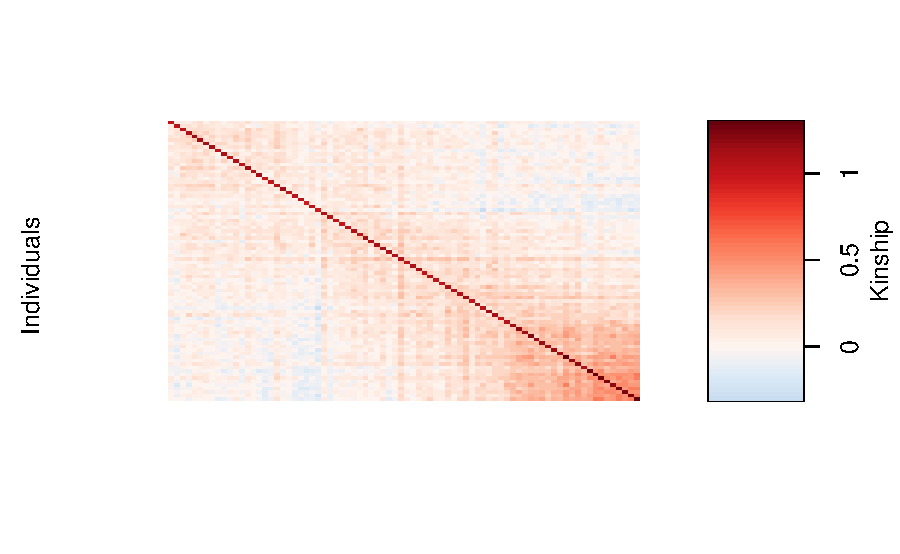
\includegraphics[width=1\linewidth]{figure/ggmix-popkin-1} 

}



\end{knitrout}

\subsection*{Fit the linear mixed model with Lasso Penalty}

We will use the most basic call to the main function of this package, which is called \texttt{ggmix}. This function will by default fit a $L_1$ penalized linear mixed model (LMM) for 100 distinct values of the tuning parameter $\lambda$. It will choose its own sequence:

\begin{knitrout}\scriptsize
\definecolor{shadecolor}{rgb}{0.969, 0.969, 0.969}\color{fgcolor}\begin{kframe}
\begin{alltt}
\hlstd{fit} \hlkwb{<-} \hlkwd{ggmix}\hlstd{(}\hlkwc{x} \hlstd{= admixed}\hlopt{$}\hlstd{xtrain,}
                 \hlkwc{y} \hlstd{= admixed}\hlopt{$}\hlstd{ytrain,}
                         \hlkwc{kinship} \hlstd{= admixed}\hlopt{$}\hlstd{kin_train)}
\hlkwd{names}\hlstd{(fit)}
\end{alltt}
\begin{verbatim}
##  [1] "result"       "ggmix_object" "n_design"     "p_design"     "lambda"      
##  [6] "coef"         "b0"           "beta"         "df"           "eta"         
## [11] "sigma2"       "nlambda"      "cov_names"    "call"
\end{verbatim}
\begin{alltt}
\hlkwd{class}\hlstd{(fit)}
\end{alltt}
\begin{verbatim}
## [1] "lassofullrank" "ggmix_fit"
\end{verbatim}
\end{kframe}
\end{knitrout}

We can see the solution path for each variable by calling the \texttt{plot} method for objects of class \texttt{ggmix\_fit}:

\begin{knitrout}\scriptsize
\definecolor{shadecolor}{rgb}{0.969, 0.969, 0.969}\color{fgcolor}\begin{kframe}
\begin{alltt}
\hlkwd{plot}\hlstd{(fit)}
\end{alltt}
\end{kframe}

{\centering 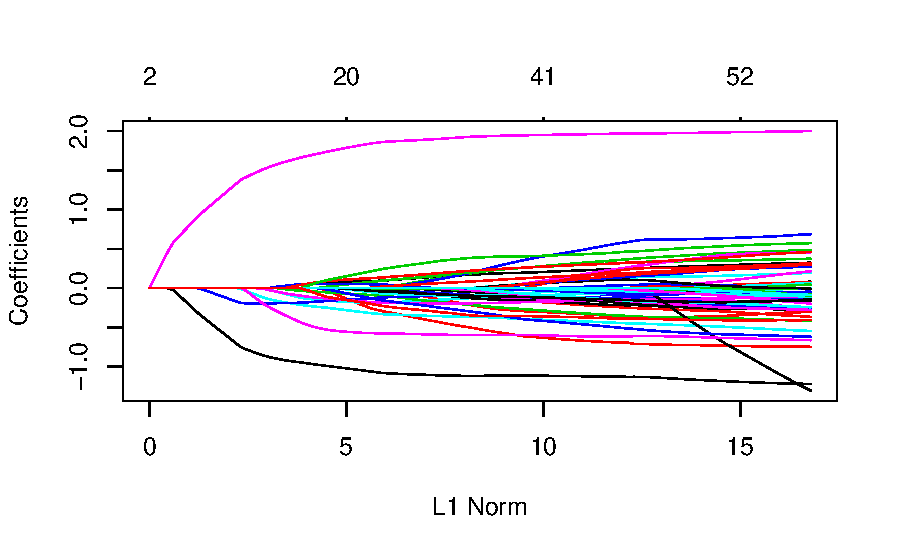
\includegraphics[width=1\linewidth]{figure/ggmix-solution-path-1} 

}



\end{knitrout}

We can also get the coefficients for given value(s) of lambda using the \texttt{coef} method for objects of class \texttt{ggmix\_fit}:

\begin{knitrout}\scriptsize
\definecolor{shadecolor}{rgb}{0.969, 0.969, 0.969}\color{fgcolor}\begin{kframe}
\begin{alltt}
\hlcom{# only the first 5 coefficients printed here for brevity}
\hlkwd{coef}\hlstd{(fit,} \hlkwc{s} \hlstd{=} \hlkwd{c}\hlstd{(}\hlnum{0.1}\hlstd{,}\hlnum{0.02}\hlstd{))[}\hlnum{1}\hlopt{:}\hlnum{5}\hlstd{, ]}
\end{alltt}
\begin{verbatim}
## 5 x 2 Matrix of class "dgeMatrix"
##                       1            2
## (Intercept) -0.03715135  0.247105426
## X23          0.00000000  0.098030248
## X36          0.00000000 -0.013022250
## X38          0.00000000  0.005378361
## X40          0.00000000  0.004028934
\end{verbatim}
\end{kframe}
\end{knitrout}
Here, \texttt{s} specifies the value(s) of $\lambda$ at which the extraction is made. The function uses linear interpolation to make predictions for values of \texttt{s} that do not coincide with the lambda sequence used in the fitting algorithm.

We can also get predictions ($X\widehat{\boldsymbol{\beta}}$) using the \texttt{predict} method for objects of class \texttt{ggmix\_fit}:

\begin{knitrout}\scriptsize
\definecolor{shadecolor}{rgb}{0.969, 0.969, 0.969}\color{fgcolor}\begin{kframe}
\begin{alltt}
\hlcom{# need to provide x to the predict function}
\hlcom{# predict for the first 5 subjects}
\hlkwd{predict}\hlstd{(fit,} \hlkwc{s} \hlstd{=} \hlkwd{c}\hlstd{(}\hlnum{0.1}\hlstd{,}\hlnum{0.02}\hlstd{),} \hlkwc{newx} \hlstd{= admixed}\hlopt{$}\hlstd{xtest[}\hlnum{1}\hlopt{:}\hlnum{5}\hlstd{,])}
\end{alltt}
\begin{verbatim}
##                1           2
## id26  2.30208546  2.45597763
## id39  0.87334032  1.62931898
## id45 -0.12296837 -0.06075786
## id52 -0.03715135 -0.97519671
## id53 -0.21046107 -0.23151040
\end{verbatim}
\end{kframe}
\end{knitrout}


\subsection*{Find the Optimal Value of the Tuning Parameter}

We use the Generalized Information Criterion (GIC) to select the optimal value for $\lambda$. The default is $a_n = log(log(n)) * log(p)$ which corresponds to a high-dimensional BIC (HDBIC):

\begin{knitrout}\scriptsize
\definecolor{shadecolor}{rgb}{0.969, 0.969, 0.969}\color{fgcolor}\begin{kframe}
\begin{alltt}
\hlcom{# pass the fitted object from ggmix to the gic function:}
\hlstd{hdbic} \hlkwb{<-} \hlkwd{gic}\hlstd{(fit)}
\hlkwd{class}\hlstd{(hdbic)}
\end{alltt}
\begin{verbatim}
## [1] "ggmix_gic"     "lassofullrank" "ggmix_fit"
\end{verbatim}
\begin{alltt}
\hlcom{# we can also fit the BIC by specifying the an argument}
\hlstd{bicfit} \hlkwb{<-} \hlkwd{gic}\hlstd{(fit,} \hlkwc{an} \hlstd{=} \hlkwd{log}\hlstd{(}\hlkwd{length}\hlstd{(admixed}\hlopt{$}\hlstd{ytrain)))}
\end{alltt}
\end{kframe}
\end{knitrout}

We can plot the HDBIC values against $\log(\lambda)$ using the \texttt{plot} method for objects of class \texttt{ggmix\_gic}:

\begin{knitrout}\scriptsize
\definecolor{shadecolor}{rgb}{0.969, 0.969, 0.969}\color{fgcolor}\begin{kframe}
\begin{alltt}
\hlkwd{plot}\hlstd{(hdbic)}
\end{alltt}
\end{kframe}

{\centering 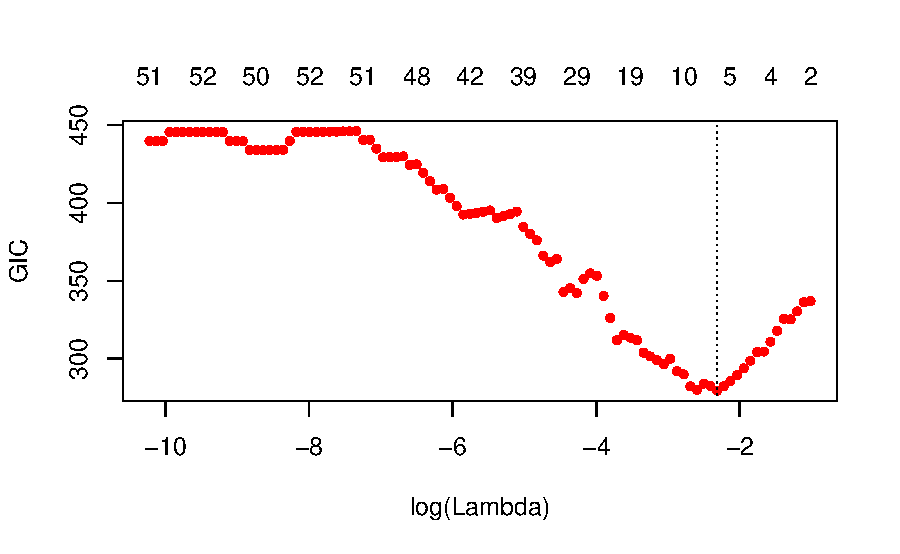
\includegraphics[width=1\linewidth]{figure/ggmix-hdbic-1} 

}



\end{knitrout}

The optimal value for $\lambda$ according to the HDBIC, i.e., the $\lambda$ that leads to the minium HDBIC is:

\begin{knitrout}\scriptsize
\definecolor{shadecolor}{rgb}{0.969, 0.969, 0.969}\color{fgcolor}\begin{kframe}
\begin{alltt}
\hlstd{hdbic[[}\hlstr{"lambda.min"}\hlstd{]]}
\end{alltt}
\begin{verbatim}
## [1] 0.09862269
\end{verbatim}
\end{kframe}
\end{knitrout}


We can also plot the BIC results:

\begin{knitrout}\scriptsize
\definecolor{shadecolor}{rgb}{0.969, 0.969, 0.969}\color{fgcolor}\begin{kframe}
\begin{alltt}
\hlkwd{plot}\hlstd{(bicfit,} \hlkwc{ylab} \hlstd{=} \hlstr{"BIC"}\hlstd{)}
\end{alltt}
\end{kframe}

{\centering 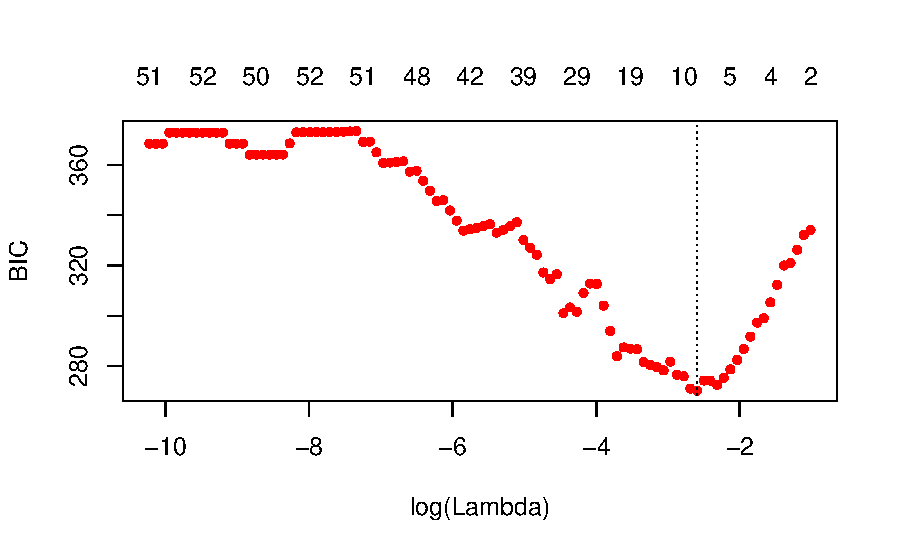
\includegraphics[width=1\linewidth]{figure/ggmix-bic-1} 

}


\begin{kframe}\begin{alltt}
\hlstd{bicfit[[}\hlstr{"lambda.min"}\hlstd{]]}
\end{alltt}
\begin{verbatim}
## [1] 0.07460445
\end{verbatim}
\end{kframe}
\end{knitrout}


\subsection*{Get Coefficients Corresponding to Optimal Model}

We can use the object outputted by the \texttt{gic} function to extract the coefficients corresponding to the selected model using the \texttt{coef} method for objects of class \texttt{ggmix\_gic}:

\begin{knitrout}\scriptsize
\definecolor{shadecolor}{rgb}{0.969, 0.969, 0.969}\color{fgcolor}\begin{kframe}
\begin{alltt}
\hlkwd{coef}\hlstd{(hdbic)[}\hlnum{1}\hlopt{:}\hlnum{5}\hlstd{, ,} \hlkwc{drop} \hlstd{=} \hlnum{FALSE}\hlstd{]}
\end{alltt}
\begin{verbatim}
## 5 x 1 sparse Matrix of class "dgCMatrix"
##                       1
## (Intercept) -0.03660806
## X23          .         
## X36          .         
## X38          .         
## X40          .
\end{verbatim}
\end{kframe}
\end{knitrout}

We can also extract just the nonzero coefficients which also provide the estimated variance components $\eta$ and $\sigma^2$:

\begin{knitrout}\scriptsize
\definecolor{shadecolor}{rgb}{0.969, 0.969, 0.969}\color{fgcolor}\begin{kframe}
\begin{alltt}
\hlkwd{coef}\hlstd{(hdbic,} \hlkwc{type} \hlstd{=} \hlstr{"nonzero"}\hlstd{)}
\end{alltt}
\begin{verbatim}
##                       1
## (Intercept) -0.03660806
## X302        -0.17607392
## X524         1.34951500
## X538        -0.72052613
## eta          0.99000000
## sigma2       1.60476289
\end{verbatim}
\end{kframe}
\end{knitrout}

We can also make predictions from the \texttt{hdbic} object, which by default will use the model corresponding to the optimal tuning parameter:

\begin{knitrout}\scriptsize
\definecolor{shadecolor}{rgb}{0.969, 0.969, 0.969}\color{fgcolor}\begin{kframe}
\begin{alltt}
\hlkwd{predict}\hlstd{(hdbic,} \hlkwc{newx} \hlstd{= admixed}\hlopt{$}\hlstd{xtest[}\hlnum{1}\hlopt{:}\hlnum{5}\hlstd{,])}
\end{alltt}
\begin{verbatim}
##                1
## id26  2.31027410
## id39  0.86922183
## id45 -0.12814532
## id52 -0.03660806
## id53 -0.21268198
\end{verbatim}
\end{kframe}
\end{knitrout}


\subsection*{Extracting Random Effects}

The user can compute the random effects using the provided \texttt{ranef} method for objects of class \texttt{ggmix\_gic}. This command will compute the estimated random effects for each subject using the parameters of the selected model:

\begin{knitrout}\scriptsize
\definecolor{shadecolor}{rgb}{0.969, 0.969, 0.969}\color{fgcolor}\begin{kframe}
\begin{alltt}
\hlkwd{ranef}\hlstd{(hdbic)[}\hlnum{1}\hlopt{:}\hlnum{5}\hlstd{]}
\end{alltt}
\begin{verbatim}
## [1] -2.4889655  1.1834200 -0.5641832 -0.9310334 -0.3458703
\end{verbatim}
\end{kframe}
\end{knitrout}



\subsection*{Diagnostic Plots}

We can also plot some standard diagnotic plots such as the observed vs. predicted response, QQ-plots of the residuals and random effects and the Tukey-Anscombe plot. These can be plotted using the \texttt{plot} method on a \texttt{ggmix\_gic} object as shown below.


\subsubsection*{Observed vs. Predicted Response}

\begin{knitrout}\scriptsize
\definecolor{shadecolor}{rgb}{0.969, 0.969, 0.969}\color{fgcolor}\begin{kframe}
\begin{alltt}
\hlkwd{plot}\hlstd{(hdbic,} \hlkwc{type} \hlstd{=} \hlstr{"predicted"}\hlstd{,} \hlkwc{newx} \hlstd{= admixed}\hlopt{$}\hlstd{xtrain,} \hlkwc{newy} \hlstd{= admixed}\hlopt{$}\hlstd{ytrain)}
\end{alltt}
\end{kframe}

{\centering 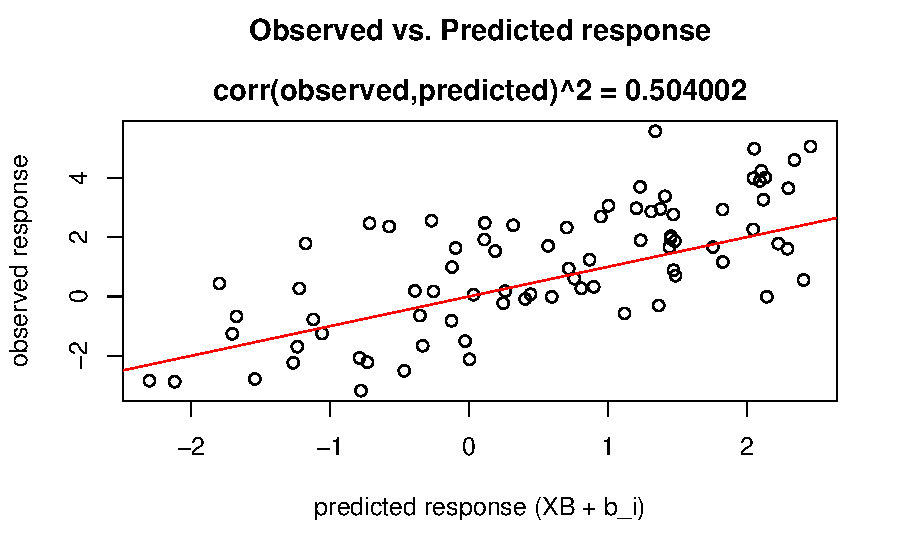
\includegraphics[width=1\linewidth]{figure/ggmix-obs-pred-1} 

}



\end{knitrout}


\subsubsection*{QQ-plots for Residuals and Random Effects}

\begin{knitrout}\scriptsize
\definecolor{shadecolor}{rgb}{0.969, 0.969, 0.969}\color{fgcolor}\begin{kframe}
\begin{alltt}
\hlkwd{plot}\hlstd{(hdbic,} \hlkwc{type} \hlstd{=} \hlstr{"QQranef"}\hlstd{,} \hlkwc{newx} \hlstd{= admixed}\hlopt{$}\hlstd{xtrain,} \hlkwc{newy} \hlstd{= admixed}\hlopt{$}\hlstd{ytrain)}
\end{alltt}
\end{kframe}

{\centering 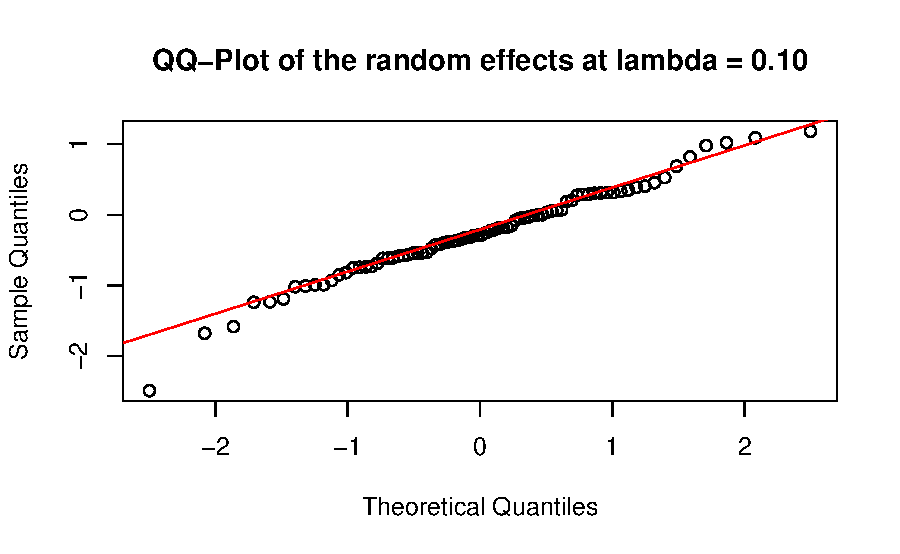
\includegraphics[width=1\linewidth]{figure/ggmix-qqplot-1} 

}


\begin{kframe}\begin{alltt}
\hlkwd{plot}\hlstd{(hdbic,} \hlkwc{type} \hlstd{=} \hlstr{"QQresid"}\hlstd{,} \hlkwc{newx} \hlstd{= admixed}\hlopt{$}\hlstd{xtrain,} \hlkwc{newy} \hlstd{= admixed}\hlopt{$}\hlstd{ytrain)}
\end{alltt}
\end{kframe}

{\centering 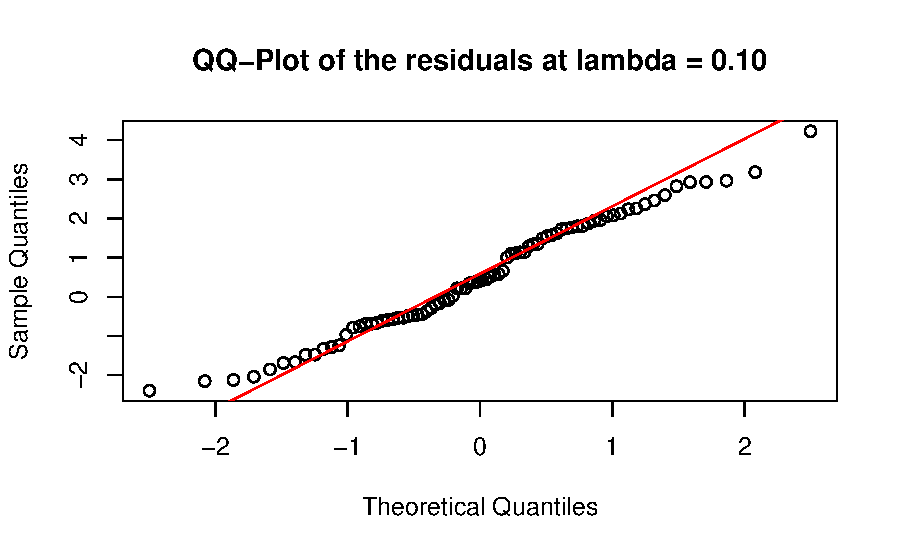
\includegraphics[width=1\linewidth]{figure/ggmix-qqplot-2} 

}



\end{knitrout}


\subsubsection*{Tukey-Anscombe Plot}

\begin{knitrout}\scriptsize
\definecolor{shadecolor}{rgb}{0.969, 0.969, 0.969}\color{fgcolor}\begin{kframe}
\begin{alltt}
\hlkwd{plot}\hlstd{(hdbic,} \hlkwc{type} \hlstd{=} \hlstr{"Tukey"}\hlstd{,} \hlkwc{newx} \hlstd{= admixed}\hlopt{$}\hlstd{xtrain,} \hlkwc{newy} \hlstd{= admixed}\hlopt{$}\hlstd{ytrain)}
\end{alltt}
\end{kframe}

{\centering 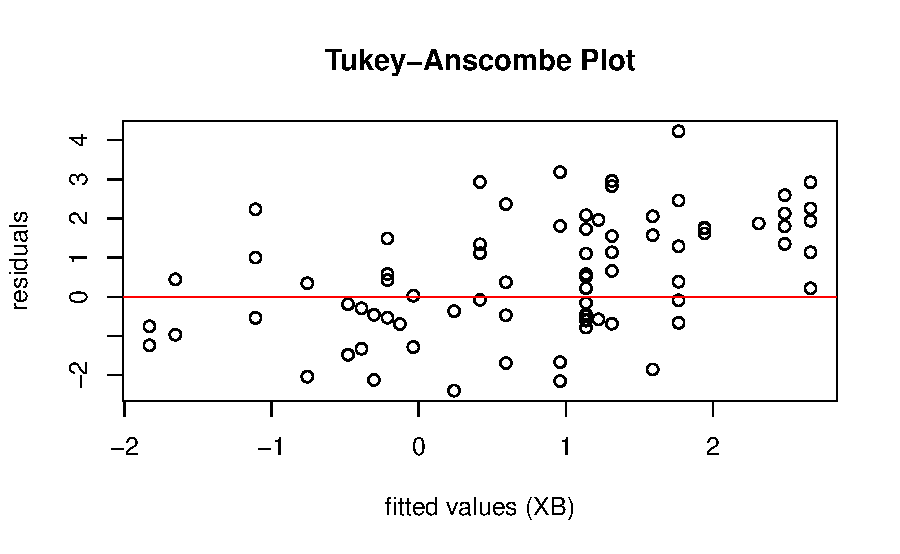
\includegraphics[width=1\linewidth]{figure/ggmix-tukey-1} 

}



\end{knitrout}


%\bibliographystyle{unsrt}
%\bibliography{GEbib}

%\bibliographystyle{unsrt}

\newpage

\bibliographystyle{vancouver}
\bibliography{ggmixbib}




\end{document}

\section{Low rank similarity matrix}

Let $\mb{K} \in \mathbb{R}^{N_T\times k}$ be the matrix containing the $k$ SNPs used to compute the factored kinship matrix $\bPhi$ given by
\begin{equation}
	\bPhi = \mb{K}\mb{K}^T \label{eq:factored}
\end{equation}

%If we let $\mb{U} \mb{\widetilde{S}} \mb{V}^T$ be the singular value decomposition (SVD) of $\mb{K}$. Then
%\begin{align*}
%\bPhi &= \left(\mb{U} \mb{\widetilde{S}} \mb{V}^T\right)\left(\mb{U} \mb{\widetilde{S}} \mb{V}^T\right)^T \\
%& = \mb{U}\mb{\widetilde{S}}\mb{V}^T\mb{V}\mb{\widetilde{S}}\mb{U}^T\\
%& = \mb{U} \mb{\widetilde{S}}\mb{\widetilde{S}}\mb{U}^T \\
%& = \mb{U} \mb{S} \mb{U}^T
%\end{align*}
%where $\mb{S}_{ii} = \mb{\widetilde{S}}_{ii}\mb{\widetilde{S}}_{ii}$. Therefore, $\mb{U}$ consists of the eigenvectors of $\bPhi$ and the eigenvalues of $\bPhi$ are given by %$\mb{\widetilde{S}}_{ii}^2$ which are the square of the eigenvalues of the SNP matrix $\mb{K} \in \mathbb{R}^{n\times p}$.
%Note that the eigenvectors of $\bPhi$ are equal to the singular vectors of $\mb{K}$, and the eigenvalues of $\bPhi$ are equal to the square of the singular values of %$\mb{K}$~\citep{berrar2003practical}.

Furthermore, let $\mb{K} = \mb{U} \bLambda \mb{V}^T$ be the singular value decomposition (SVD) of $\mb{K}$. Plugging this into~\eqref{eq:factored} we get
\begin{align}
	\bPhi &= \left(\mb{U} \bLambda \mb{V}^T\right)\left(\mb{U} \bLambda \mb{V}^T\right)^T \nonumber\\
	& = \mb{U}\bLambda\mb{V}^T\mb{V}\bLambda\mb{U}^T \nonumber\\
	& = \mb{U} \bLambda\bLambda\mb{U}^T \nonumber\\
	& = \mb{U} \bSigma \mb{U}^T, \label{eq:svdphi}
\end{align}
Therefore, the eigenvectors of $\bPhi$ are equal to the singular vectors of $\mb{K}$ (denoted by $\bU$), and the eigenvalues of $\bPhi$ (denoted by the diagonal matrix $\bSigma$) are equal to the square of the singular values of $\mb{K}$~\citep{berrar2003practical}. This allows us to bypass the explicit computation of the kinship matrix by directly applying SVD on the SNP matrix $\bW$. ~\cite{lippert2011fast} noted that the computational time for fitting the LMM can be reduced if the matrix $\mb{K}$ is not full rank, i.e., when $k < N_T$. This is due to the fact that the matrix $\bD_{N_T \times N_T}$ contains $k$ non-zero eigenvalues followed by $N_T-k$ zeros on the diagonal. Let $\bU \equiv \left[\bU_1 \,\, \bU_2\right]$, where $\bU_1 \in \mathbb{R}^{N_T\times k}$ and $\bU_2 \in \mathbb{R}^{N_T \times (n-k)}$ are  the matrices of singular vectors corresponding to the $k$ non-zero and $N_T-k$ zero eigenvalues, respectively. Then~\eqref{eq:svdphi} can be written as
\begin{equation}
	\bPhi = \bU_1 \bSigma \bU_1^T
\end{equation}
%Following~\cite{lippert2011fast}, we show that the log-likelihood~\eqref{eq:Likelihood} can be expressed in terms of $\bU_1$ only, foregoing the need to compute $\bU_2$.
We now try to simplify the log-likelihood~\eqref{eq:Likelihood}. Since there are $N_T-k$ zero eigenvalues, the second term in~\eqref{eq:Likelihood} reduces to
\begin{equation}
	\frac{1}{2} \left(  \sum_{i=1}^{k} \log(1 + \eta (\Sigma_i-1)) + (N_T-k) \log(1-\eta)\right) \label{eq:term2}
\end{equation}
where $\Sigma_i = \Lambda_i^2$, and $\Lambda_i$ is the $i^{\tm{th}}$ singular value of $\bW$. Let $a \equiv (\bY - \bX \bbeta)$. The third term in~\eqref{eq:Likelihood} can be written as
\begin{align}
	\frac{1}{2\sigma^2} a^T \left[ \eta \bPhi + (1-\eta)\bI_n \right] ^{-1} a &= \frac{1}{2\sigma^2} a^T \left[ \eta \bU_1 \bSigma_1 \bU_1^T + (1-\eta)\bI_n \right] ^{-1} a  \nonumber \\
	& = \frac{1}{2\sigma^2} a^T \left[ \bC \bB \bC^T + \mb{A} \right] ^{-1} a \nonumber
\end{align}
where
\begin{align*}
	\mb{A} & = (1-\eta) \bI_n \\
	\mb{B} & = \bSigma_1 \\
	\mb{C} & = \sqrt{\eta} \bU_1 \\
	\mb{C}^T & = \sqrt{\eta} \bU_1^T
\end{align*}
Assuming $\bC \bB \bC^T + \mb{A}$ is non-singular, the inverse of $\left[ \bC \bB \bC^T + \mb{A} \right]$ is given explicitly by the Woodbury formula~\citep{golub2012matrix}
\begin{align}
	\left(\bA + \bC \bB \bC^T\right)^{-1} & = \bA^{-1} - \bA^{-1} \bC \left(\bB^{-1} + \bC^T\bA^{-1} \bC\right)^{-1}\bC^T \bA^{-1} \label{eq:woodbury}
\end{align}
Substituting the values for $\bA, \bB$ and $\bC$ into~\eqref{eq:woodbury} we get
\begin{align}
	\left(\bA + \bC \bB \bC^T\right)^{-1} & = \frac{1}{1-\eta}\bI_{N_T} - \frac{\sqrt{\eta}}{1-\eta}\bI_{N_T}\bU_1 \left(\bSigma_1^{-1} + \frac{\eta}{1-\eta}\bU_1^T \bI_{N_T} \bU\right)^{-1}\frac{\sqrt{\eta}}{1-\eta}\bU_1^T \bI_{N_T} \nonumber \\
	& = \frac{1}{1-\eta} \left[ \bI_{N_T} - \frac{\eta}{1-\eta}\bU_1 \left(\bSigma_1^{-1} + \frac{\eta}{1-\eta}\bI_{k} \right)^{-1}\bU_1^T \right] \nonumber \\
	& = \frac{1}{1-\eta} \left[ \bI_{N_T} - \frac{\eta}{1-\eta}\bU_1 \left(\frac{\eta}{1-\eta} \left(\frac{1-\eta}{\eta}\bSigma_1^{-1} + \bI_{k}\right) \right)^{-1}\bU_1^T \right] \nonumber \\
	& = \frac{1}{1-\eta} \left[ \bI_{N_T} - \bU_1 \left(\frac{1-\eta}{\eta}\bSigma_1^{-1} + \bI_{k}\right) ^{-1}\bU_1^T \right] \label{eq:term3}
\end{align}


where we have used the following identities: $\bI_k = \bU_1^T\bU_1$, $\bI_{N_T -k} = \bU_2^T\bU_2$.
%, and
%\begin{align}
%\bI_{N_T} & = \bU \bU^T  \nonumber\\
%& =\left[\bU_1 \,\, \bU_2\right] \left[\bU_1 \,\, \bU_2\right] ^T \nonumber\\
%& = \bU_1 \bU_1^T + \bU_2 \bU_2^T \label{eq:In} \nonumber
%\end{align}

Substituting~\eqref{eq:term2} and~\eqref{eq:term3} in~\eqref{eq:Likelihood} we obtain
\begin{align}
	\begin{split}
		-\ell(\bTheta) & \propto \frac{N_T}{2}\log(\sigma^2) + \frac{1}{2} \left(  \sum_{i=1}^{k} \log(1 + \eta (\Sigma_i-1)) + (N_T-k) \log(1-\eta)\right) + \\
		&\frac{1}{2} \left\lbrace \left(\bY - \bX\bbeta \right)^T  \left[\frac{1}{\sigma^2(1-\eta)}\left(  \bI_{N_T} - \bU_1 \left(\frac{1-\eta}{\eta}\bSigma_1^{-1} + \bI_{k}\right) ^{-1}\bU_1^T \right)  \right] \left(\bY - \bX\bbeta \right)  \right\rbrace
	\end{split} \label{eq:loglikrowrank}
\end{align}

\section{Group Lasso with Low-rank Similarity Matrix}
This section focuses on the part of the log-likelihood~\eqref{eq:loglikrowrank} that depends on $\bbeta$.

\subsection{Model}
Only the third term of the log-likelihood~\eqref{eq:loglikrowrank} depends on $\bbeta$:
\begin{equation}
	\frac{1}{2} \left\lbrace \left(\bY - \bX\bbeta \right)^T  \left[\frac{1}{\sigma^2(1-\eta)}\left(  \bI_{N_T} - \bU_1 \left(\frac{1-\eta}{\eta}\bSigma_1^{-1} + \bI_{k}\right) ^{-1}\bU_1^T \right)  \right] \left(\bY - \bX\bbeta \right)  \right\rbrace \label{eq:likeW}
\end{equation}
Equation~\eqref{eq:likeW} can be written more generally as
\[
L(\bbeta\mid\bD)=\frac{1}{2}\left[\bY-\widehat{\bY}\right]^{\top}\mathbf{W}\left[\bY-\widehat{\bY}\right]
\]
where $\widehat{\bY}=\sum_{j=1}^{p}\beta_{j}X_{j}$, $\bD$ is the working data $\lbrace \bY, \bX \rbrace$, and $\bW$ is an $N_T \times N_T$ weight matrix given by
\begin{equation}
	\bW = \frac{1}{\sigma^2(1-\eta)}\left(  \bI_{N_T} - \bU_1 \left(\frac{1-\eta}{\eta}\bSigma_1^{-1} + \bI_{k}\right) ^{-1}\bU_1^T \right)   \label{eq:weight}
\end{equation}

%Consider the linear regression problem where we have a continuous response $\by\in\mathbb{R}^{n}$
%and let $\bX$ be the design matrix with $n$ rows and $p$ columns where $n$ is the sample size of the raw data. If an intercept is used in the model, we let the first column of $\bX$ be a vector of 1.
Assume that we the predictors in the design matrix $\bX \in \mathbb{R}^{N_T \times p}$ belong to $K$ groups and that the group membership is already defined such that $(1,2,\ldots,p)=\bigcup_{k=1}^{K}I_{k}$ and the cardinality of index set $I_{k}$ is $p_{k}$, $I_{k}\bigcap I_{k^{\prime}}=\emptyset$ for $k\neq k^{\prime},1\le k,k^{\prime}\le K$. Thus group $k$ contains $p_{k}$ predictors, which are $x_{j}$'s for $j\in I_{k}$, and $1\le k\le K.$ If an intercept is included, then $I_{1}=\{1\}$. Given the group partition, we use $\bbeta_{(k)}$ to denote the segment of $\bbeta$ corresponding to group $k$. This notation is used for any $p$-dimensional vector.
%In a more compact form, and introducing observation weights
%\[
%L(\bbeta\mid\bD)=\frac{1}{2}\left[Y-\hat{Y}\right]^{\top}\mathbf{W}\left[Y-\hat{Y}\right]
%\]
%where $\hat{Y}=\sum_{j=1}^{p}\beta_{j}X_{j}$, $\bD$ is the working data $\lbrace \by, \bX \rbrace$, $\bW$ is an $N_T \times N_T$ weight matrix. Then the problem we consider can be expressed as
We consider the group lasso penalized estimator
\begin{equation}
	\min_{\bbeta}L(\bbeta \mid \bD)+\lambda\sum_{k=1}^{K}w_{k}\|\bbk\|_{2},\label{eq:wlslasso}
\end{equation}

The loss function $L$ satisfies the quadratic majorization (QM) condition, since there exists
a $p\times p$ matrix $\bH=\bX^{\trans}\mathbf{W}\bX$, and $\nabla L(\bbeta|\bD)=-\left(Y-\hat{Y}\right)^{\top}\mathbf{W}\bX$, which may only depend on the data $\bD$, such that for all $\bbeta,\bbeta^{*}$,
\begin{equation}
	L(\bbeta\mid\bD)\le L(\bbeta^{*}\mid\bD)+(\bbeta-\bbeta^{*})^{\trans}\nabla L(\bbeta^{*}|\bD)+\frac{1}{2}(\bbeta-\bbeta^{*})^{\trans}\bH(\bbeta-\bbeta^{*}).\label{QM1}
\end{equation}

\subsection{Algorithm}

Noticing that the penalty term $\sum_{k=1}^{K}w_{k}||\bbeta_{(k)}||_{2}$ is separable with respect to the indices of the features $k=1, \ldots, K$, we can derive the \textit{groupwise-majorization-descent} (GMD) algorithm for computing the solution of~\eqref{eq:wlslasso} when the loss function satisfies the QM condition. Let $\widetilde{\bbeta}$ denote the current solution of $\bbeta$. Without loss of generality, let us derive the GMD update of $\bbkt$, the coefficients of group $k$. Define $\bH_{k}$ as the sub-matrix of $\bH$ corresponding to group $k$. For example, if group 2 is $\{2,4\}$ then $\bH_{(2)}$ is a $2\times2$ matrix with
\[
\bH_{(2)}=\left[\begin{array}{cc}
h_{2,2} & h_{2,4}\\
h_{4,2} & h_{4,4}
\end{array}\right],
\]

where $h_{i,j}$ is the $i,j$th entry of the $\bH$ matrix. Write $\bbeta$ such that $\bbeta_{(k^{\prime})}=\widetilde{\bbeta}_{(k^{\prime})}$ for $k^{\prime}\ne k$. Given $\bbeta_{(k^{\prime})}=\widetilde{\bbeta}_{(k^{\prime})}$ for $k^{\prime}\ne k$, the optimal $\bbk$ is defined as
\begin{equation}
	\arg\min_{\boldsymbol{\beta}^{(k)}}L(\bbeta\mid\bD)+\lambda w_{k}\Vert\bbk\Vert_{2}.\label{GMDeq1}
\end{equation}
Unfortunately, there is no closed form solution to~\eqref{GMDeq1} for a general loss function with general design matrix. We overcome the computational obstacle by taking advantage of the QM condition. From~\eqref{QM1} we have
\[
L(\bbeta\mid\bD)\le L(\widetilde{\bbeta}\mid\bD)+(\bbeta-\widetilde{\bbeta})^{\trans}\nabla L(\widetilde{\bbeta}|\bD)+\frac{1}{2}(\bbeta-\widetilde{\bbeta})^{\trans}\bH(\bbeta-\widetilde{\bbeta}).
\]

Write $U(\widetilde{\bbeta})=-\nabla L(\widetilde{\bbeta}|\bD)$. Using
\[
\bbeta-\widetilde{\bbeta}=(\underbrace{0,\ldots,0}_{k-1},\bbk-\bbkt,\underbrace{0,\ldots,0}_{K-k}),
\]
we can write
\begin{equation}
	L(\bbeta\mid\bD)\le L(\widetilde{\bbeta}\mid\bD)-(\bbk-\bbkt)^{\trans}U_{(k)}+\frac{1}{2}(\bbk-\bbkt)^{\trans}\bH_{(k)}(\bbk-\bbkt).\label{GMDeq2}
\end{equation}
where
\begin{align}
	U_{(k)} & =\frac{\partial}{\partial\bbk}L_{Q}(\bbeta\mid\bD)=-\left(Y-\hat{Y}\right)^{\top}\mathbf{W}\mathbf{X}_{(k)},\label{eq:gradientj-1}\\
	\mathbf{H}_{(k)} & =\frac{\partial^{2}}{\partial\bbk\partial\bbk^{\top}}L_{Q}(\bbeta\mid\bD)=\mathbf{X}_{(k)}^{\top}\mathbf{W}\mathbf{X}_{(k)}.\label{eq:hessianj-1}
\end{align}

Let $\eta_{k}$ be the largest eigenvalue of $\bH_{(k)}$. We set $\gamma_{k}=(1+\varepsilon^{*})\eta_{k}$, where $\varepsilon^{*}=10^{-6}$. Then we can further relax the upper bound in~\eqref{GMDeq2} as
\begin{equation}
	L(\bbeta\mid\bD)\leq L(\widetilde{\bbeta}\mid\bD)-(\bbeta^{(k)}-\widetilde{\bbeta}^{(k)})^{\trans}U_{(k)}+\frac{1}{2}\gamma_{k}(\bbeta^{(k)}-\widetilde{\bbeta}^{(k)})^{\trans}(\bbeta^{(k)}-\widetilde{\bbeta}^{(k)}).\label{GMDeq3-1}
\end{equation}
It is important to note that the inequality strictly holds unless for $\bbeta^{(k)}=\widetilde{\bbeta}^{(k)}$. Instead of minimizing~\eqref{GMDeq1} we solve
\begin{equation}
	\arg\min_{\bbeta^{(k)}}L(\widetilde{\bbeta}\mid\bD)-(\bbeta^{(k)}-\widetilde{\bbeta}^{(k)})^{\trans}U_{(k)}+\frac{1}{2}\gamma_{k}(\bbeta^{(k)}-\widetilde{\bbeta}^{(k)})^{\trans}(\bbeta^{(k)}-\widetilde{\bbeta}^{(k)})+\lambda w_{k}\Vert\bbeta^{(k)}\Vert_{2}.\label{GMDeq4-1}
\end{equation}

Denote by $\widetilde{\bbeta}^{(k)}(\textrm{new})$ the solution to~\eqref{GMDeq4-1}. It is straightforward to see that $\widetilde{\bbeta}^{(k)}(\textrm{new})$ has a simple closed-from expression
\begin{equation}
	\widetilde{\bbeta}^{(k)}(\textrm{new})=\frac{1}{\gamma_{k}}\left(U^{(k)}+\gamma_{k}\widetilde{\bbeta}^{(k)}\right)\left(1-\frac{\lambda w_{k}}{\Vert U^{(k)}+\gamma_{k}\widetilde{\bbeta}^{(k)}\Vert_{2}}\right)_{+}.\label{GMDeq5-1}
\end{equation}

Algorithm~\ref{alg1} summarizes the details of GMD.

\begin{algorithm}
	\begin{enumerate}
		\item For $k=1,\ldots,K$, compute $\gamma_k$, the largest eigenvalue of $\bH^{(k)}$.
		\item Initialize $\widetilde \bbeta$.
		\item Repeat the following cyclic groupwise updates until convergence:
		\begin{enumerate}
			\item[---] for $k=1,\ldots,K$, do step (3.1)--(3.3)
			\begin{enumerate}
				\item[3.1]
				Compute $U(\widetilde \bbeta )=-\nabla L(\widetilde \bbeta | \bD)$.
				\item[3.2]
				Compute
				$
				\widetilde \bbeta^{(k)}(\textrm{new}) = \frac{1}{\gamma_k}\left( U^{(k)}+\gamma_k \widetilde \bbeta^{(k)} \right)\left(1-\frac{\lambda w_k}{\Vert U^{(k)}+\gamma_k \widetilde \bbeta^{(k)} \Vert_2}\right)_{+} .
				$
				\item[3.3]
				Set $\widetilde \bbeta^{(k)}=\widetilde \bbeta^{(k)}(\textrm{new})$.
			\end{enumerate}
		\end{enumerate}
	\end{enumerate}
	\caption{The GMD algorithm for general group-lasso learning. \label{alg1}}
\end{algorithm}


\subsection{Convergence}

We can prove the strict descent property of GMD by using the MM principle \citep{MM1,hunter2004tutorial,MM08}. Define
\begin{equation}
	Q(\bbeta \mid \bD)=L(\widetilde \bbeta \mid \bD)-(\bbeta^{(k)}-\widetilde \bbeta^{(k)})^{\trans}
	U^{(k)}+\frac{1}{2} \gamma_k (\bbeta^{(k)}-\widetilde \bbeta^{(k)})^{\trans} ( \bbeta^{(k)}- \widetilde \bbeta^{(k)})+\lambda w_k \Vert \bbeta^{(k)}\Vert_2.
\end{equation}
Obviously, $Q(\bbeta \mid \bD)=L(\bbeta \mid \bD)+\lambda w_k \Vert \bbeta^{(k)}\Vert_2$ when $\bbeta^{(k)}=\widetilde \bbeta^{(k)}$ and
(\ref{GMDeq3}) shows that
$Q(\bbeta \mid \bD) > L(\bbeta \mid \bD)+\lambda w_k \Vert \bbeta^{(k)}\Vert_2$ when $\bbeta^{(k)} \neq \widetilde \bbeta^{(k)}$.
After updating $\widetilde \bbeta^{(k)}$ using (\ref{GMDeq5}), we have
\begin{eqnarray*}
	L(\widetilde \bbeta^{(k)}(\textrm{new}) \mid \bD)+\lambda w_k \Vert \widetilde \bbeta^{(k)}(\textrm{new}) \Vert_2
	&  \le &  Q(\widetilde \bbeta^{(k)}(\textrm{new})  \mid \bD)\\
	& \le & Q(\widetilde \bbeta  \mid \bD) \\
	& = & L(\widetilde \bbeta \mid \bD)+\lambda w_k \Vert \widetilde \bbeta^{(k)}\Vert_2.
\end{eqnarray*}
Moreover, if $\widetilde \bbeta^{(k)}(\textrm{new}) \neq \widetilde \bbeta^{(k)}$, then the first inequality becomes
\begin{eqnarray*}
	L(\widetilde \bbeta^{(k)}(\textrm{new}) \mid \bD)+\lambda w_k \Vert \widetilde \bbeta^{(k)}(\textrm{new}) \Vert_2
	&  < &  Q(\widetilde \bbeta^{(k)}(\textrm{new})  \mid \bD).
\end{eqnarray*}
Therefore, the objective function is strictly decreased after updating all groups in a cycle, unless the solution does not change after each groupwise update. If this is the case,
we can show that the solution must satisfy the KKT conditions, which means that the algorithm converges and finds the right answer. To see this,
if $\widetilde \bbeta^{(k)}(\textrm{new}) = \widetilde \bbeta^{(k)}$ for all $k$, then by the update formula \eqref{GMDeq5-1} we have that for all $k$
\begin{align}\label{KKTcond1}
	\widetilde \bbeta^{(k)} = \frac{1}{\gamma_k}\left( U^{(k)}+\gamma_k \widetilde \bbeta^{(k)} \right)\left(1-\frac{\lambda w_k}{\Vert U^{(k)}+\gamma_k \widetilde \bbeta^{(k)} \Vert_2}\right) \qquad\textrm{if }\Vert U^{(k)}+\gamma_k \widetilde \bbeta^{(k)} \Vert_2 > \lambda w_{k},\\\label{KKTcond2}
	\widetilde \bbeta^{(k)} = \boldsymbol{0} \qquad\textrm{if }\Vert U^{(k)}+\gamma_k \widetilde \bbeta^{(k)} \Vert_2 \leq \lambda w_{k}.
\end{align}
By straightforward algebra  we obtain the KKT conditions:
\begin{align*}
	-U^{(k)}+\lambda w_{k}\cdot\frac {\widetilde\bbeta^{(k)} }{\Vert\widetilde\bbeta^{(k)}\Vert_2}=\boldsymbol{0}\qquad\textrm{if }\widetilde\bbeta^{(k)}\neq \boldsymbol{0},\\
	\left\Vert
	U^{(k)}
	\right\Vert_2 \le\lambda w_{k}\qquad\textrm{if }\widetilde\bbeta^{(k)}=\boldsymbol{0},
\end{align*}
where $k=1,2,\ldots,K$. Therefore, if the objective function stays unchanged after a cycle, the algorithm necessarily converges to the right
answer.




\subsection{Fitting Options and Algorithms}
Recall $\mb{K} \in \mathbb{R}^{N_T\times k}$ is the matrix containing the $k$ SNPs used to compute the factored kinship matrix $\bPhi$. The dimension of this matrix will determine the algorithm used as shown in the table below.
\ctable[caption={Algorithm used based on dimension of $\mb{K}$. },label=tab:review,pos=h!,doinside=\footnotesize]{LLLLL}{
}{
\FL
Dimension of $\mb{K}$    & lasso   & group lasso \ML
$N_T > k$  			& gcdnet (or degenerate gglasso)  & gglasso (GMD Algorithm with weight matrix) \\
$N_T < k$              & glmnet (Coordinate descent with observation weights)   & gglasso (GMD Algorithm with observation weights)
\LL
}
